This chapter presents the architecture of JOP and the motivation
behind the various different design decisions we faced. The first
sections give an overview of JOP, describe the microcode and the
pipeline.

Pipelined instruction processing calls for high memory bandwidth.
Caches are needed in order to avoid bottlenecks resulting from the
main memory bandwidth. As seen in Chapter~\ref{chap:java}, there are
two memory areas that are frequently accessed by the JVM: the stack
and the method area. In this chapter, time-predictable cache
solutions for both areas that are implemented in JOP are presented.

\section{Overview of JOP}

This section gives an overview of JOP architecture.
Figure~\ref{fig:arch:jop:block} shows JOP's major function units. A
typical configuration of JOP contains the processor core, a memory
interface and a number of IO devices. The module extension provides
the link between the processor core, and the memory and IO modules.

\begin{figure}[t]
    \centering
    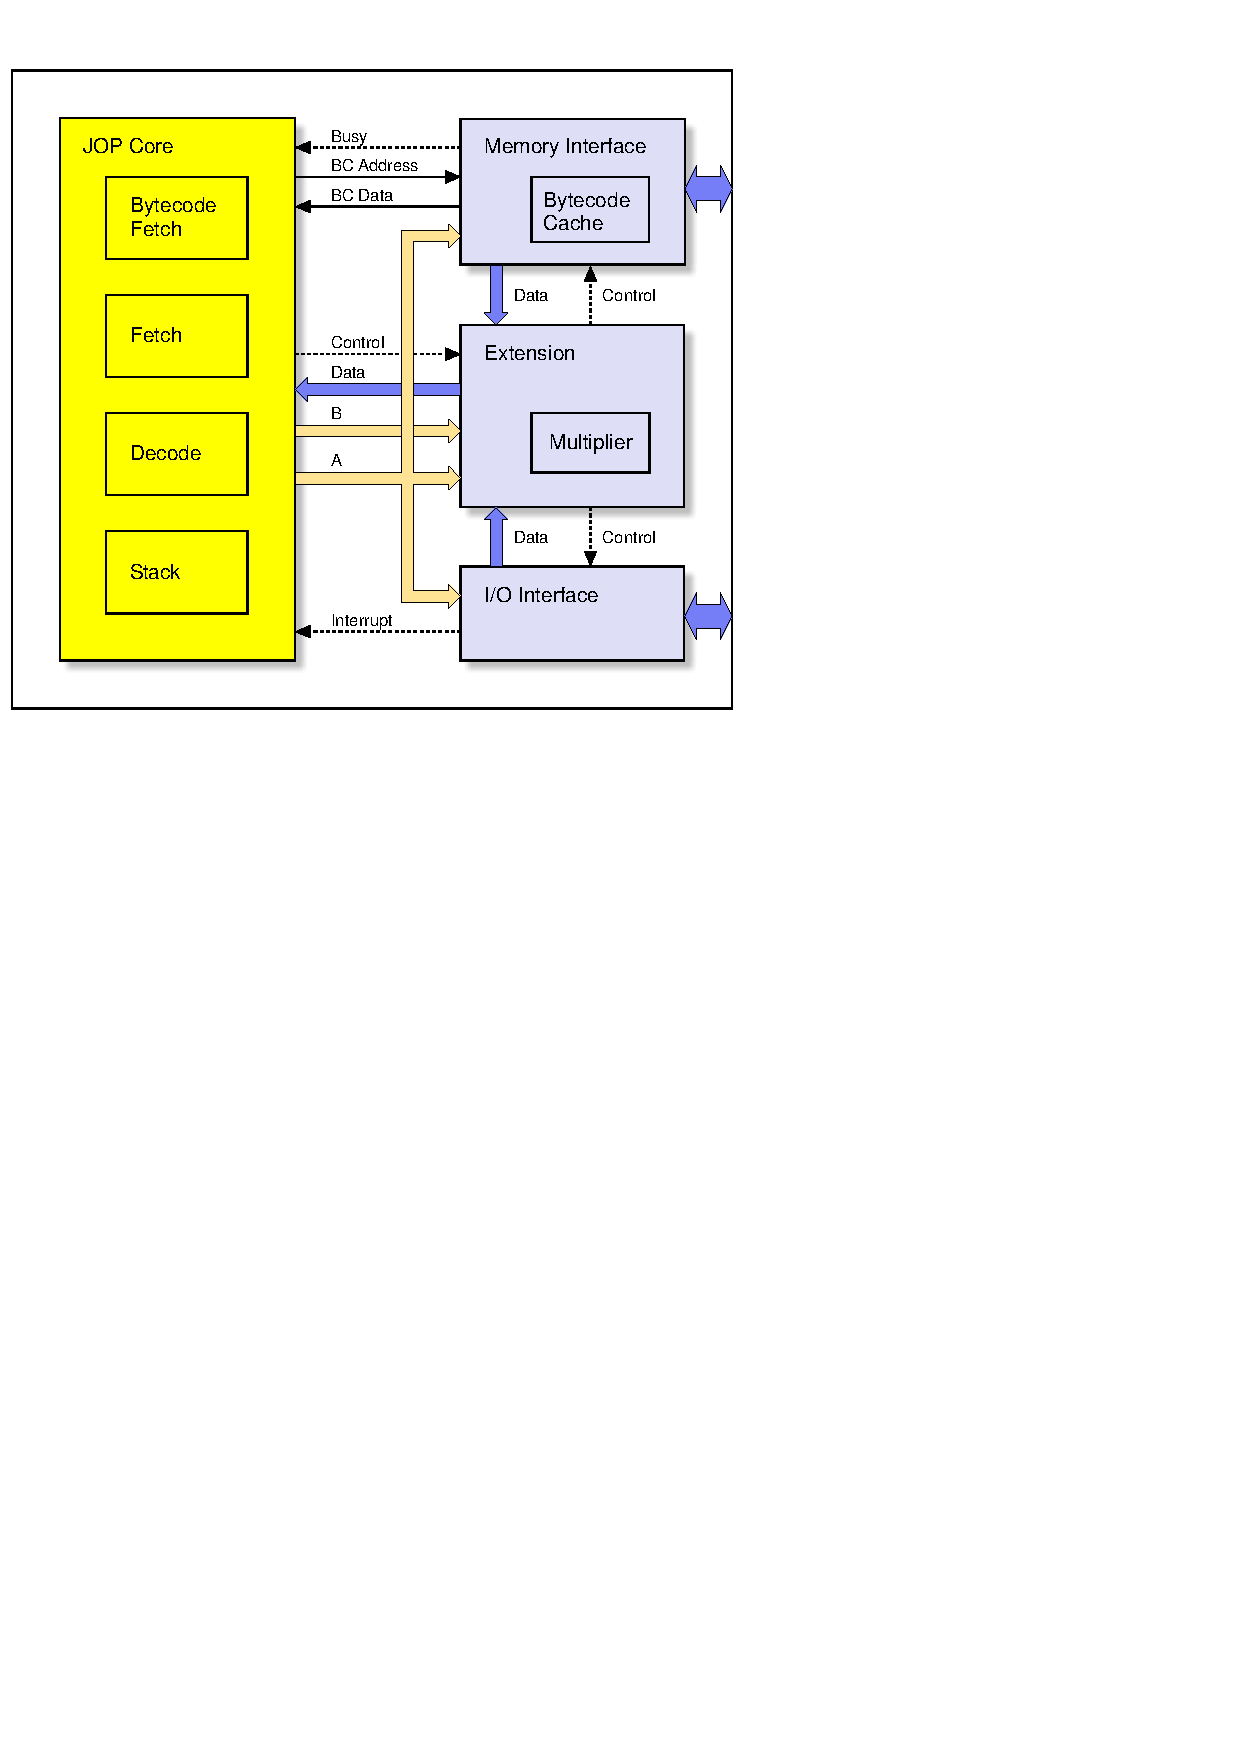
\includegraphics{arch/arch_jop_block}
    \caption{Block diagram of JOP}
    \label{fig:arch:jop:block}
\end{figure}


The processor core contains the three microcode pipeline stages
\emph{microcode fetch}, \emph{decode} and \emph{execute} and an
additional translation stage \emph{bytecode fetch}. The ports to the
other modules are the two top elements of the stack (A and B), input
to the top-of-stack (Data), bytecode cache address and data, and a
number of control signals. There is no direct connection between the
processor core and the external world.

The memory controller implements the simple memory load and store
operations and the field and array access bytecodes. It also contains
the method cache. The memory interface provides a connection between
the main memory and the memory controller. The extension module
controls data read and write. The \emph{busy} signal is used by the
microcode instruction \code{wait}\footnote{The busy signal can also
be used to stall the whole processor pipeline. This was the change
made to JOP by Flavius Gruian \cite{jop:sac05}. However, in this
synchronization mode, the concurrency between the memory access
module and the main pipeline is lost.} to synchronize the processor
core with the memory unit. The core reads bytecode instructions
through dedicated buses (BC address and BC data) from the memory
controller. The request for a method to be placed in the cache is
performed through the extension module, but the cache hit detection
and load is performed by the memory controller independently of the
processor core (and therefore concurrently).

The I/O interface contains peripheral devices, such as the system
time and timer interrupt for real-time thread scheduling, a serial
interface and application-specific devices. Read and write to and
from this module are controlled by the memory controller. All
external devices\footnote{The external device can be as simple as a
line driver for the serial interface that forms part of the interface
module, or a complete bus interface, such as the ISA bus used to
connect e.g.\ an Ethernet chip.} are connected to the I/O interface.

The extension module performs two functions: (a) it contains hardware
accelerators (such as the multiplier unit in this example) and (b)
the multiplexer for the read data that is loaded into the
top-of-stack register. The write data from the top-of-stack (A) is
connected directly to all modules.

The division of the processor into those modules greatly simplifies
the adaptation of JOP for different application domains or hardware
platforms. Porting JOP to a new FPGA board usually results in changes
in the memory interface alone. Using the same board for different
applications only involves making changes to the I/O interface. JOP
has been ported to several different FPGAs and prototyping boards and
has been used in different real-world applications (see
Chapter~\ref{chap:results}), but it never proved necessary to change
the processor core.

\section{Microcode}
\label{sec:microcode}

The following discussion concerns two different instruction sets:
\emph{bytecode} and \emph{microcode}. Bytecodes are the instructions
that make up a compiled Java program. These instructions are
executed by a Java virtual machine. The JVM does not assume any
particular implementation technology. Microcode is the native
instruction set for JOP. Bytecodes are translated, during their
execution, into JOP microcode. Both instruction sets are designed
for an extended\footnote{An extended stack machine is one in which
there are instructions available to access elements deeper down in
the stack.} stack machine.

\subsection{Translation of Bytecodes to Microcode}

To date, no hardware implementation of the JVM exists that is
capable of executing \emph{all} bytecodes in hardware alone. This is
due to the following: some bytecodes, such as \code{new}, which
creates and initializes a new object, are too complex to implement
in hardware. These bytecodes have to be emulated by software.

To build a self contained JVM without an underlying operating
system, direct access to the memory and I/O devices is necessary.
There are no bytecodes defined for low-level access. These low-level
services are usually implemented in \emph{native} functions, which
means that another language (C) is native to the processor. However,
for a Java processor, bytecode is the \emph{native} language.

One way to solve this problem is to implement simple bytecodes in
hardware and to emulate the more complex and \emph{native} functions
in software with a different instruction set (sometimes called
microcode). However, a processor with two different instruction sets
results in a complex design.

Another common solution, used in Sun's picoJava \cite{pjMicroArch},
is to execute a subset of the bytecode native and to use a software
trap to execute the remainder. This solution entails an overhead (a
minimum of 16 cycles in picoJava, see \ref{subsec:related:picojava})
for the software trap.

In JOP, this problem is solved in a much simpler way. JOP has a
single \emph{native} instruction set, the so-called microcode.
During execution, every Java bytecode is translated to either one,
or a sequence of microcode instructions. This translation merely
adds one pipeline stage to the core processor and results in no
execution overheads (except for a bytecode branch that takes 4
instead of 3 cycles to execute). The area overhead of the
translation stage is 290~LCs, or about 15\% of the LCs of a typical
JOP configuration. With this solution, we are free to define the JOP
instruction set to map smoothly to the stack architecture of the
JVM, and to find an instruction coding that can be implemented with
minimal hardware.

\begin{figure}
    \centering
    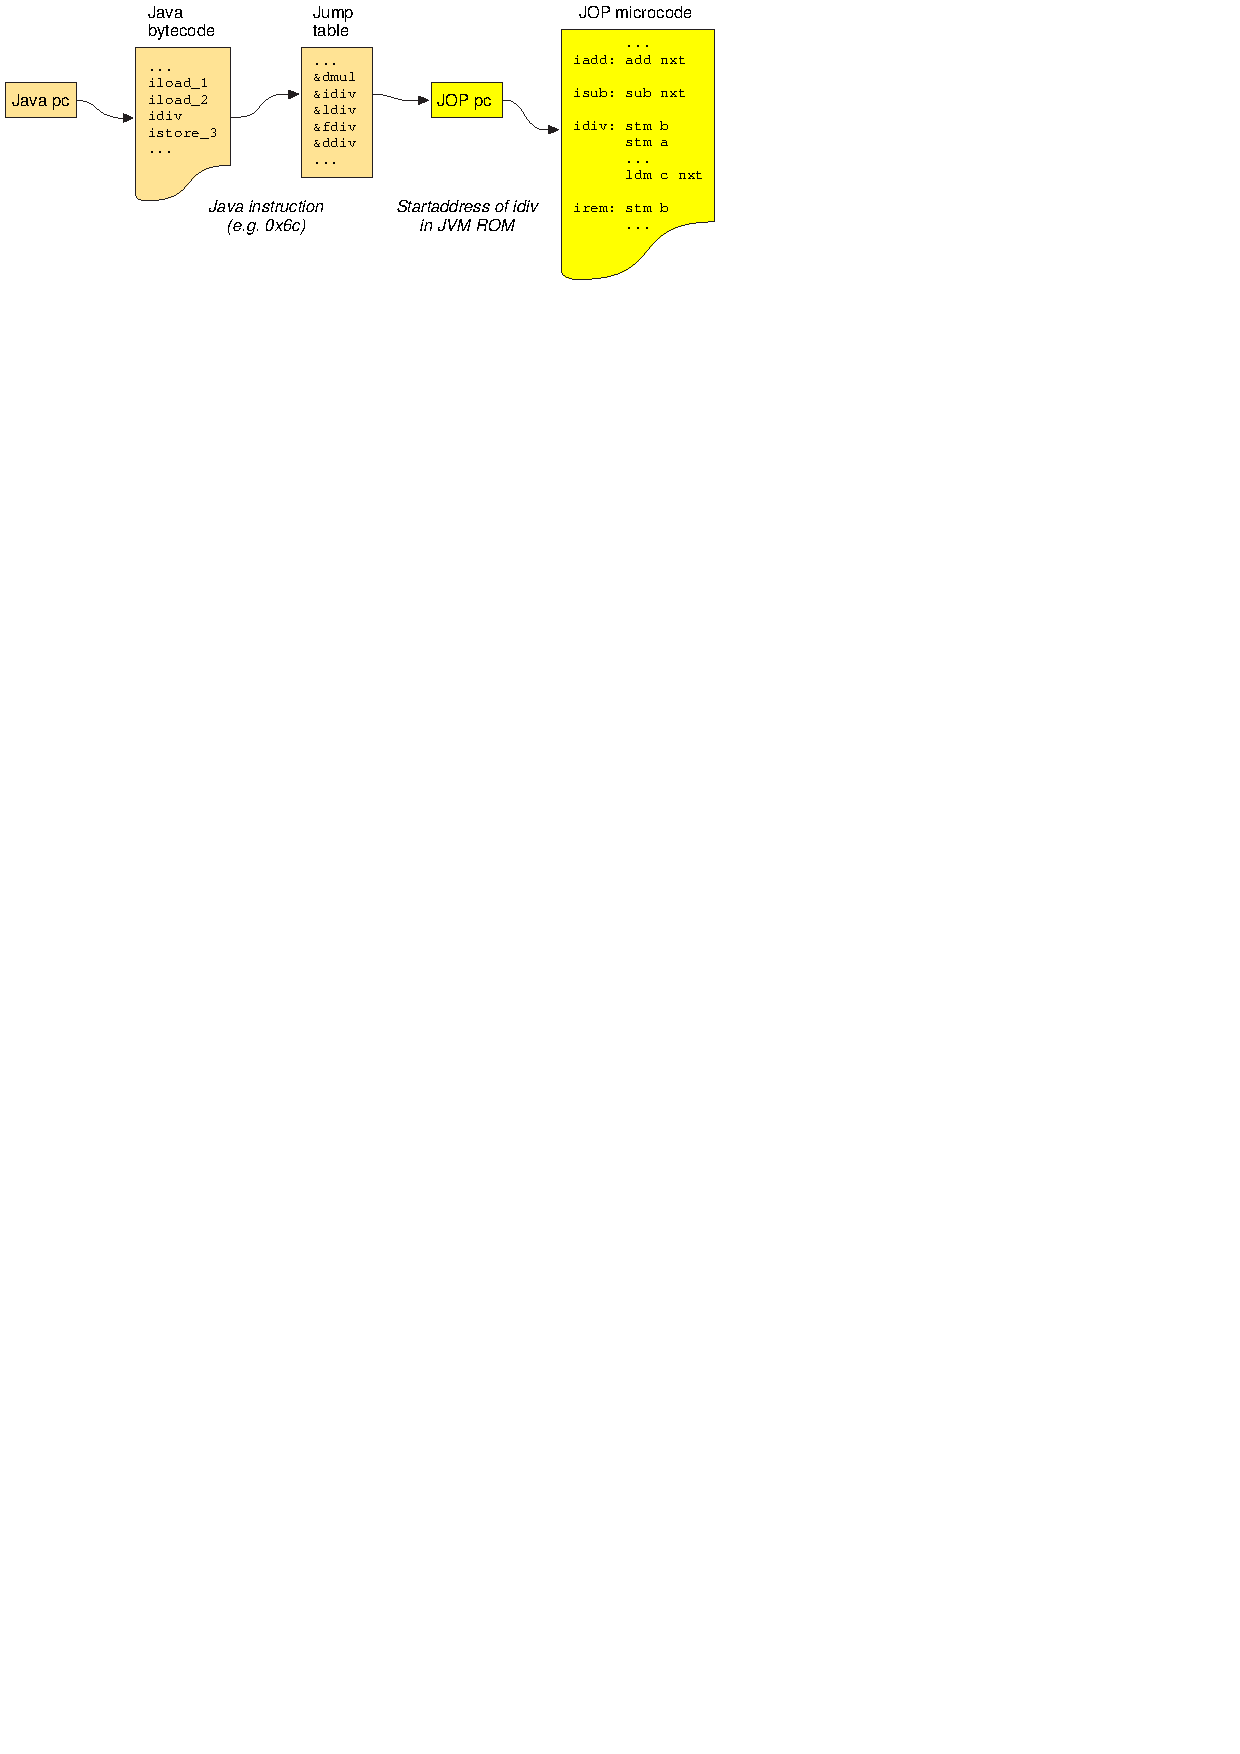
\includegraphics{arch/arch_indirection}
    \caption{Data flow from the Java program counter to JOP microcode}
    \label{fig_arch_data_flow}
\end{figure}


Figure~\ref{fig_arch_data_flow} gives an example of the data flow
from the Java program counter to JOP microcode. The figure
represents the two pipeline stages bytecode fetch/translate and
microcode fetch. The fetched bytecode acts as an index for the jump
table. The jump table contains the start addresses for the bytecode
implementation in microcode. This address is loaded into the JOP
program counter for every bytecode executed. JOP executes the
sequence of microcode until the last one. The last one is marked
with \emph{nxt} in microcode assembler. This \emph{nxt} bit in the
microcode ROM triggers a new translation i.e., a new address is
loaded into the JOP program counter. In
Figure~\ref{fig_arch_data_flow} the implementation of bytecode
\code{idiv} is an example of a longer sequence that ends with
microcode instruction \code{ldm c nxt}.

The difference to other forms of instruction translation in hardware
is that the proposed solution is time predictable. The translation
takes one cycle (one pipeline stage) for each bytecode, independent
from the execution history. Instruction folding, e.g., implemented
in picoJava \cite{pJ1,pjMicroArch}, is also a form of instruction
translation in hardware. Folding is used to translate several (stack
oriented) bytecode instructions to a RISC type instruction. This
translation needs an instruction buffer and the fill level of this
instruction buffer depends on the execution history. The length of
this history that has to be considered for analysis is not bounded.
Therefore this form of instruction translation is not exactly time
predictable.


\subsection{Compact Microcode}

For the JVM to be implemented efficiently, the microcode has to
\emph{fit} to the Java bytecode. Since the JVM is a stack machine,
the microcode is also stack-oriented. However, the JVM is not a pure
stack machine. Method parameters and local variables are defined as
\emph{locals}. These locals can reside in a stack frame of the
method and are accessed with an offset relative to the start of this
\emph{locals} area.

Additional local variables (16) are available at the microcode level.
These variables serve as scratch variables, like registers in a
conventional CPU. Furthermore, the constant pool pointer (cp), the
method pointer (mp), and pointers to the method tables of
\code{JVM.java} and \code{JVMHelp.java} are stored in these
variables. The 16 variables are located in the on-chip stack memory.
However, arithmetic and logic operations are performed on the stack.

Some bytecodes, such as ALU operations and the short form access to
\emph{locals}, are directly implemented by an equivalent microcode
instruction (with a different encoding). Additional instructions are
available to access internal registers, main memory and I/O devices.
A relative conditional branch (zero/non zero of TOS) performs control
flow decisions at the microcode level. For optimum use of the
available memory resources, all instructions are 8 bits long. There
are no variable-length instructions and every instruction, with the
exception of \code{wait}, is executed in a single cycle. To keep the
instruction set this dense, the following concept is applied:
immediate values and branch offsets are addressed through one
indirection. The instruction just contains an index for the
constants.

Two types of operands, immediate values and branch distances,
normally force an instruction set to be longer than 8 bits. The
instruction set is either expanded to 16 or 32 bits, as in typical
RISC processors, or allowed to be of variable length at byte
boundaries. A first implementation of the JVM with a 16-bit
instruction set showed that only a small number of different
constants are necessary for immediate values and relative branch
distances.

In the current realization of JOP, the different immediate values
are collected while the microcode is being assembled and are put
into the initialization file for the on-chip memory. These constants
are accessed indirectly in the same way as the local variables. They
are similar to initialized variables, apart from the fact that there
are no operations to change their value during runtime, which would
serve no purpose and would waste instruction codes.  The microcode
local variables, the microcode constants and the stack share the
same on-chip memory. Using a single memory block simplifies the
multiplexer in the execution stage.

A similar solution is used for branch distances. The assembler
generates a VHDL file with a table for all found branch constants.
This table is indexed using instruction bits during runtime. These
indirections during runtime make it possible to retain an 8-bit
instruction set, and provide 16 different immediate values and 32
different branch constants. For a general purpose instruction set,
these indirections would impose too many restrictions. As the
microcode only implements the JVM, this solution is a viable option.

To simplify the logic for instruction decoding, the instruction
coding is carefully chosen. For example, one bit in the instruction
specifies whether the instruction will increment or decrement the
stack pointer. The offset to access the \emph{locals} is directly
encoded in the instruction. This is not the case for the original
encoding of the equivalent bytecodes (e.g. \emph{iload\_0} is 0x1a
and \emph{iload\_1} is 0x1b). Whenever a multiplexer depends on an
instruction, the selection is directly encoded in the instruction.

\subsection{Instruction Set}

JOP implements 54 different microcode instructions. These
instructions are encoded in 8 bits. With the addition of the
\emph{nxt} and \emph{opd} bits in every instruction, the effective
instruction length is 10 bits.

\begin{description}
    \item[Bytecode equivalent:]
These instructions are direct implementations of bytecodes and
result in one cycle execution time for the bytecode (except
\code{st} and \code{ld}): \code{pop}, \code{and}, \code{or},
\code{xor}, \code{add}, \code{sub}, \code{st$<$n$>$}, \code{st},
\code{ushr}, \code{shl}, \code{shr}, \code{nop}, \code{ld$<$n$>$},
\code{ld}, \code{dup}

    \item[Local memory access:]
The first 16 words in the internal stack memory are reserved for
internal variables. The next 16 words contain constants. These
memory locations are accessed using the following instructions:
\code{stm}, \code{stmi}, \code{ldm}, \code{ldmi}, \code{ldi}

    \item[Register manipulation:]
The stack pointer, the variable pointer and the Java program counter
are loaded or stored with: \code{stvp}, \code{stjpc}, \code{stsp},
\code{ldvp}, \code{ldjpc}, \code{ldsp}, \code{star}

    \item[Bytecode operand:]
The operand is loaded from the bytecode RAM, converted to a 32-bit
word and pushed on the stack with: \code{ld\_opd\_8s},
\code{ld\_opd\_8u}, \code{ld\_opd\_16s}, \code{ld\_opd\_16u}

    \item[External memory access:]
The autonomous memory subsystem and the IO subsystem are accessed by
using the following instructions: \code{stmra}, \code{stmwa},
\code{stmwd}, \code{wait}, \code{ldmrd}, \code{stbcrd},
\code{ldbcstart}, \code{stald}, \code{stast}, \code{stgf},
\code{stpf}, \code{stcp}

    \item[Multiplier:]
The multiplier is accessed with: \code{stmul}, \code{ldmul}

    \item[Microcode branches:]
Two conditional branches in microcode are available: \code{bz},
\code{bnz}

    \item[Bytecode branch:]
All 17 bytecode branch instructions are mapped to one instruction:
\code{jbr}

\end{description}
%
A detailed description of the microcode instructions can be found in
Appendix~\ref{appx:jop:instr}.

\subsection{Bytecode Example}

The example in Figure~\ref{lst:arch:micro1} shows the implementation
of a single cycle bytecode and an infrequent bytecode as a sequence
of JOP instructions. The suffix \code{nxt} marks the last instruction
of the microcode sequence. In this example, the \code{iadd} bytecode
is mapped to the equivalent \code{add} microcode and executed in a
single cycle, whereas \code{swap} takes four cycles to execute, and
after the last instruction (\code{ldm b nxt}), the first instruction
for the next bytecode is executed. The scratch variables, as shown in
the second example, are stored in the on-chip memory that is shared
with the stack cache.

\begin{figure}
\begin{lstlisting}[caption={Implementation of \code{iadd} and \code{swap}},
label=lst:arch:micro1]
    iadd:   add nxt    // 1 to 1 mapping

    //  a and b are scratch variables for the
    //  JVM code.
    swap:   stm a      // save TOS in variable a
            stm b      // save TOS-1 in variable b
            ldm a      // push a on stack
            ldm b nxt  // push b on stack and fetch next bytecode
\end{lstlisting}
\end{figure}

Some bytecodes are followed by operands of between one and three
bytes in length (except \code{lookupswitch} and \code{tableswitch}).
Due to pipelining, the first operand byte that follows the bytecode
instruction is available when the first microcode instruction enters
the execution stage. If this is a one-byte long operand, it is ready
to be accessed. The increment of the Java program counter after the
read of an operand byte is coded in the JOP instruction (an
\emph{opd} bit similar to the \emph{nxt} bit).

In Listing~\ref{lst:arch:micro2}, the implementation of
\code{sipush} is shown. The bytecode is followed by a two-byte
operand. Since the access to bytecode memory is only
one\footnote{The decision is to avoid buffers that would introduce
time dependencies over bytecode boundaries.} byte per cycle,
\emph{opd} and \emph{nxt} are not allowed at the same time. This
implies a minimum execution time of $n+1$ cycles for a bytecode with
$n$ operand bytes.

\begin{figure}
\begin{lstlisting}[caption={Bytecode operand load},
label=lst:arch:micro2]
    sipush: nop opd        // fetch next byte
            nop opd        // and one more
            ld_opd_16s nxt // load 16 bit operand
\end{lstlisting}
\end{figure}

\subsection{Microcode Branches}

At the microcode level two conditional branches that test the TOS are
available: \code{bz} branch on zero, and \code{bnz} branch on not
zero. The branches are followed by two delay slots, i.e., the
following two instructions are executed independent of the branch
condition outcome. Furthermore, the branch condition is also
pipelined, i.e., it has to be available one cycle earlier.
Listing~\ref{lst:arch:micro3} shows the condition delay and the
branch delay slots.

\begin{figure}
\begin{lstlisting}[caption={Microcode condition delay and branch delay slots},
label=lst:arch:micro3]
        add            // sets the condition for the branch
        nop            // one cycle condition delay slot
        bz label       // a branch on TOS zero
        instr1         // is executed
        instr2         // is executed
        instr3         // executed on fall through
\end{lstlisting}
\end{figure}

\subsection{Flexible Implementation of Bytecodes}
\label{subsec:flex:bc}

As mentioned above, some Java bytecodes are very complex. One
solution already described is to emulate them through a sequence of
microcode instructions. However, some of the more complex bytecodes
are very seldom used. To further reduce the resource implications
for JOP, in this case local memory, bytecodes can even be
implemented by \emph{using} Java bytecodes. That means bytecodes
(e.g., \code{new} or floating point operations) can be implemented
in Java. This feature also allows for the easy configuration of
resource usage versus performance.

During the assembly of the JVM, all labels that represent an entry
point for the bytecode implementation are used to generate the
translation table. For all bytecodes for which no such label is
found, i.e.\ there is no implementation in microcode, a
\emph{not-implemented} address is generated. The instruction
sequence at this address invokes a static method from a system
class. This class contains 256 static methods, one for each possible
bytecode, ordered by the bytecode value. The bytecode is used as the
index in the method table of this system class. A single empty
static method consumes three 32-bit words in memory. Therefore, the
overhead of this special class is 3~KB, which is 9\% of a minimal
\emph{hello world} program (34~KB memory footprint). As described in
Section~\ref{sec:hwsw:co}, this feature also allows for the easy
configuration of resource usage versus performance.

\subsection{Summary}

In order to handle the great variation in the complexity of Java
bytecodes we have proposed a translation to a different instruction
set, the so-called microcode. This microcode is still an instruction
set for a stack machine, but more RISC-like than the CISC-like JVM
bytecodes.

At the time of this writing 43 of the 201 different bytecodes are
implemented by a single microcode instruction, 92 by a microcode
sequence, and 41 bytecodes are implemented in Java. Furthermore, JOP
contains additional bytecodes that are used to implement low-level
operations, such as direct memory access. Those bytecodes are mapped
to native, static methods in \code{com.jopdesign.sys.Native}. In the
next section we will see how this translation is handled in JOP's
pipeline and how it can simplify interrupt handling.


\section{The Processor Pipeline}
\label{sec:pipeline}

JOP is a fully pipelined architecture with single cycle execution of
microcode instructions and a novel approach of translation from Java
bytecode to these instructions. Figure~\ref{fig_arch_pipeline} shows
the datapath for JOP, representing the pipeline from left to right.
Blocks arranged vertically belong to the same pipeline stage.

\begin{figure}[t]
    \centering
    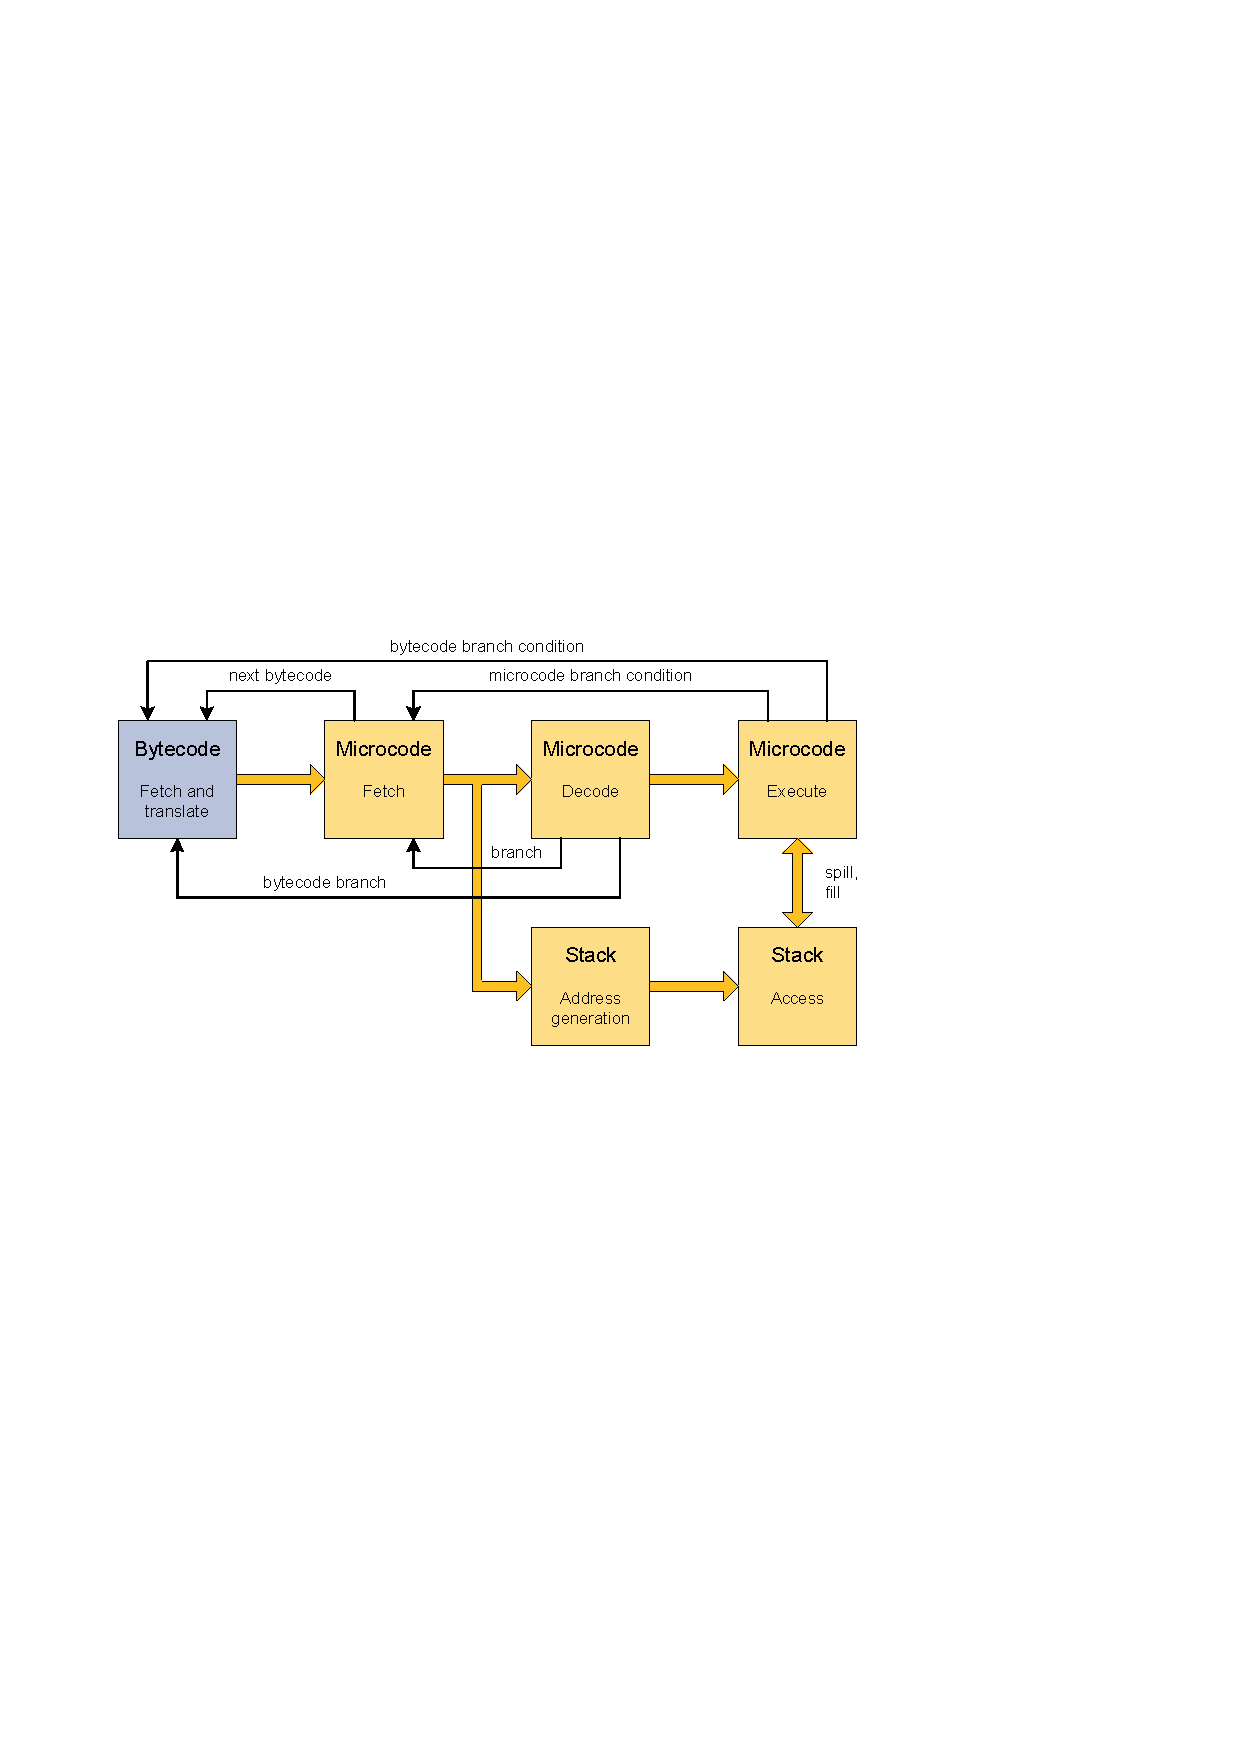
\includegraphics[scale=\picscale]{arch/arch_pipeline}
    \caption{Datapath of JOP}
    \label{fig_arch_pipeline}
\end{figure}

Three stages form the JOP core pipeline, executing microcode
instructions. An additional stage in the front of the core pipeline
fetches Java bytecodes -- the instructions of the JVM -- and
translates these bytecodes into addresses in microcode. Bytecode
branches are also decoded and executed in this stage. The second
pipeline stage fetches JOP instructions from the internal microcode
memory and executes microcode branches. Besides the usual decode
function, the third pipeline stage also generates addresses for the
stack RAM (the stack cache). As every stack machine microcode
instruction (except \code{nop}, \code{wait}, and \code{jbr}) has
either \emph{pop} or \emph{push} characteristics, it is possible to
generate fill or spill addresses for the \emph{following}
instruction at this stage. The last pipeline stage performs ALU
operations, load, store and stack spill or fill. At the execution
stage, operations are performed with the two topmost elements of the
stack.

The stack architecture allows for a short pipeline, which results in
short branch delays. Two branch delay slots are available after a
conditional microcode branch. A stack machine with two explicit
registers for the two topmost stack elements and automatic
fill/spill to the stack cache needs neither an extra write-back
stage nor any data forwarding. See Section~\ref{sec:stack} for a
detailed description.

The method cache (\emph{Bytecode Cache}), microcode ROM, and stack
RAM are implemented with single cycle access in the FPGA's internal
memories.


\subsection{Java Bytecode Fetch}

In the first pipeline stage, as shown in
Figure~\ref{fig_arch_bc_fetch}, the Java bytecodes are fetched from
the internal memory (\emph{Method cache}). The bytecode is mapped
through the translation table into the address (\emph{jpaddr}) for
the microcode ROM. Interrupts and exceptions are handled by
redirection of the microcode address to the handler code.

\begin{figure}[t]
    \centering
    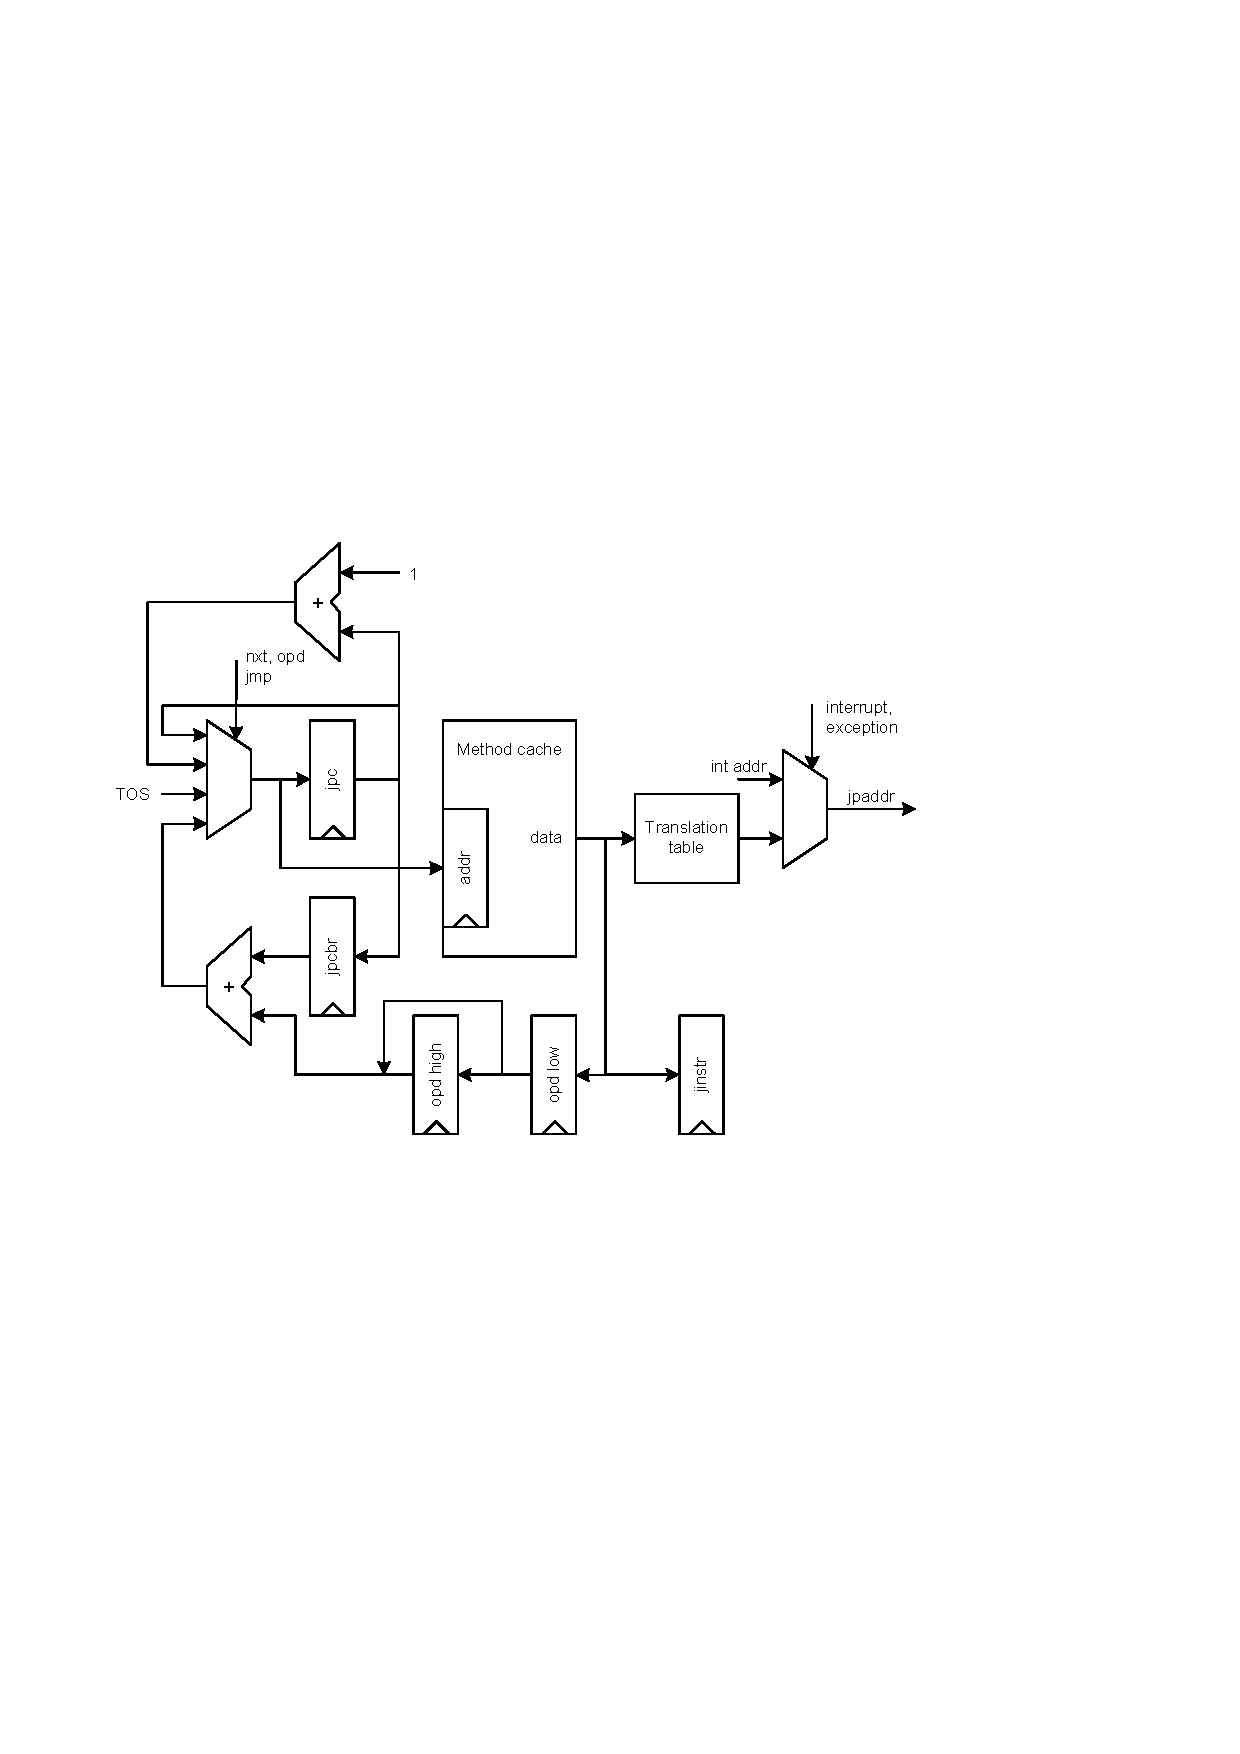
\includegraphics[scale=\picscale]{arch/arch_bcfetch}
    \caption{Java bytecode fetch and translation}
    \label{fig_arch_bc_fetch}
\end{figure}

The fetched bytecode results in an absolute jump in the microcode
(the second stage). If the bytecode is mapped one-to-one with a JOP
instruction, the following fetched bytecode again results in a jump
in the microcode in the following cycle. If the bytecode is a complex
one, JOP continues to execute microcode. At the end of this
instruction sequence, the next bytecode, and therefore the new jump
address, is requested (signal \emph{nxt}).

The method cache serves as the instruction cache and is filled on
method invoke and return. Details about this time-predictable
instruction cache can be found in Section~\ref{sec:cache}.

The bytecode is also stored in a register for later use as an
operand (requested by signal \emph{opd}). Bytecode branches are also
decoded and executed in this stage. Since \emph{jpc} is also used to
read the operands, the program counter is saved in \emph{jpcbr}
during an instruction fetch. \emph{jinstr} is used to decode the
branch type and \emph{jpcbr} to calculate the branch target address.

\subsection{JOP Instruction Fetch}

The second pipeline stage, as shown in Figure~\ref{fig_arch_fetch},
fetches JOP instructions from the internal microcode memory and
executes microcode branches.

\begin{figure}
    \centering
    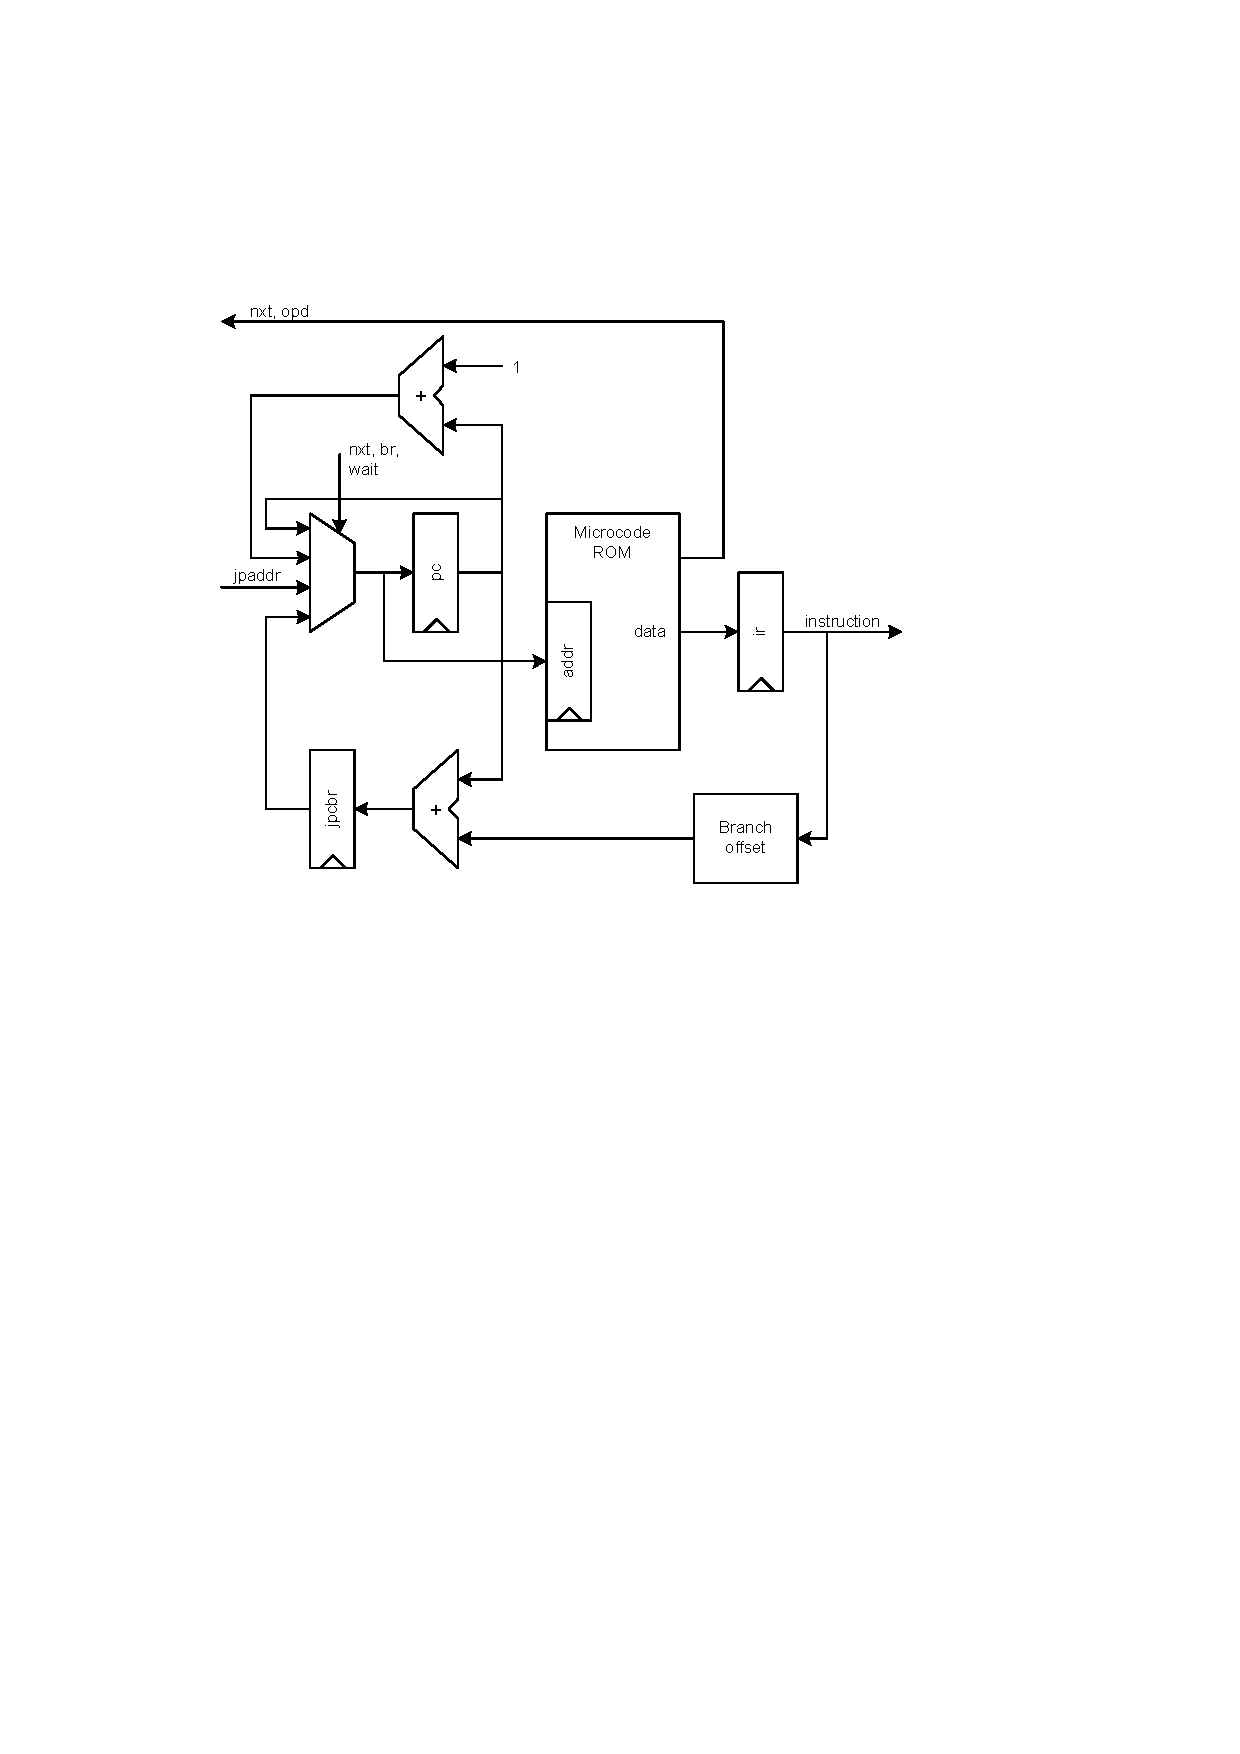
\includegraphics[scale=\picscale]{arch/arch_fetch}
    \caption{JOP instruction fetch}
    \label{fig_arch_fetch}
\end{figure}

The JOP microcode, which implements the JVM, is stored in the
microcode ROM. The program counter \emph{pc} is incremented during
normal execution. If the instruction is labeled with \emph{nxt} a
new bytecode is requested from the first stage and \emph{pc} is
loaded with \emph{jpaddr}. \emph{jpaddr} is the starting address for
the implementation of that bytecode. The label \emph{nxt} is the
flag that marks the end of the microcode instruction stream for one
bytecode. Another flag, \emph{opd}, indicates that a bytecode
operand needs to be fetched in the first pipeline stage. Both flags
are stored in a table that is indexed by the program counter.

\emph{brdly} contains the target address for a conditional branch.
The same offset is shared by a number of branch destinations. A
table (\emph{branch offset}) is used to store these relative
offsets. This indirection means that only 5 bits need to be used in
the instruction coding for branch targets and thereby allow greater
offsets. The three tables \emph{BC fetch table}, \emph{branch
offset} and \emph{translation table} (from the bytecode fetch stage)
are generated during the assembly of the JVM code. The outputs are
plain VHDL files. For an implementation in an FPGA, recompiling the
design after changing the JVM implementation is a straightforward
operation. For an ASIC with a loadable JVM, it is necessary to
implement a different solution.

FPGAs available to date do not allow asynchronous memory access.
They therefore force us to use the registers in the memory blocks.
However, the output of these registers is not accessible. To avoid
having to create an additional pipeline stage just for a
register-register move, the read address register of the microcode
ROM is clocked on the negative edge.

An alternative solution for this problem would be to use the output
of the multiplexer for the \emph{pc} and the read address register
of the memory. However, this solution results in a longer critical
path, as the multiplexer can no longer be combined with the
flip-flops that form the \emph{pc} in the same LCs. This is an
example of how implementation technology (the FPGA) can influence
the architecture.

\subsection{Decode and Address Generation}

Besides the usual decode function, the third pipeline, as shown in
Figure~\ref{fig_arch_decode}, also generates addresses for the stack
RAM.

\begin{figure}
    \centering
    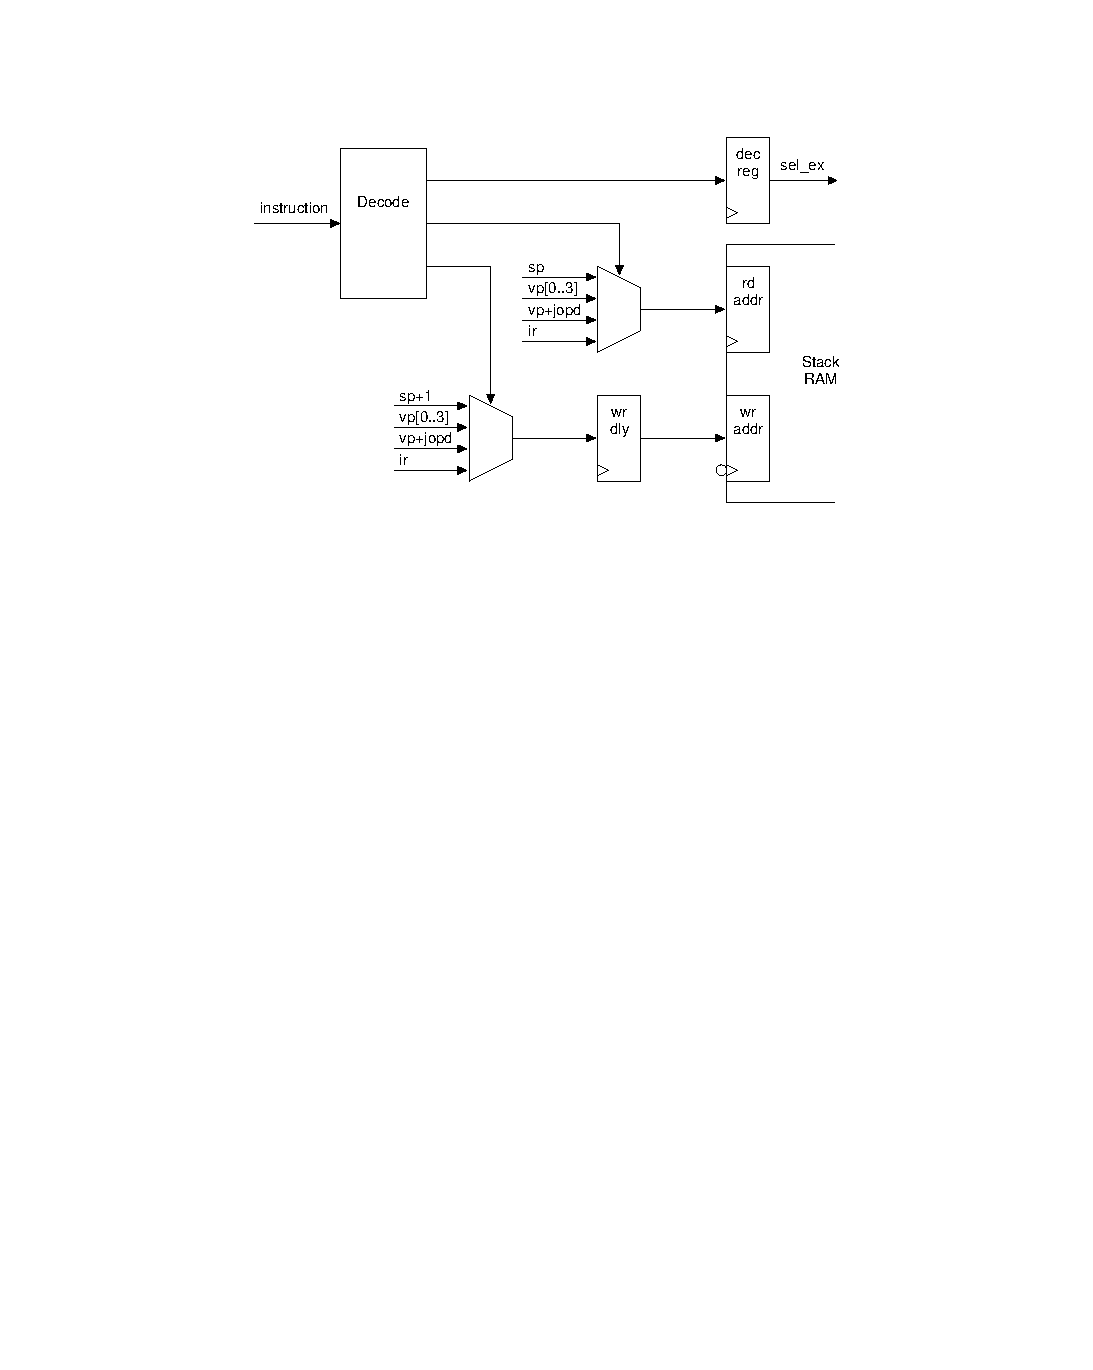
\includegraphics[scale=\picscale]{arch/arch_decaddr}
    \caption{Decode and address generation}
    \label{fig_arch_decode}
\end{figure}


As we can see in Section~\ref{sec:stack}
Table~\ref{tab_stack_address}, read and write addresses are either
relative to the stack pointer or to the variable pointer. The
selection of the pre-calculated address can be performed in the
decode stage. When an address relative to the stack pointer is used
(either as read or as write address, never for both) the stack
pointer is also decremented or incremented in the decode stage.

Stack machine instructions can be categorized from a stack
manipulation perspective as either \emph{pop} or \emph{push}. This
allows us to generate fill or spill TOS-1 addresses for the
\emph{following} instruction during the decode stage, thereby saving
one extra pipeline stage.

\subsection{Execute}

At the execution stage, as shown in Figure~\ref{fig_arch_exe},
operations are performed using two discrete registers: TOS and
TOS-1, labeled \emph{A} and \emph{B}.

\begin{figure}
    \centering
    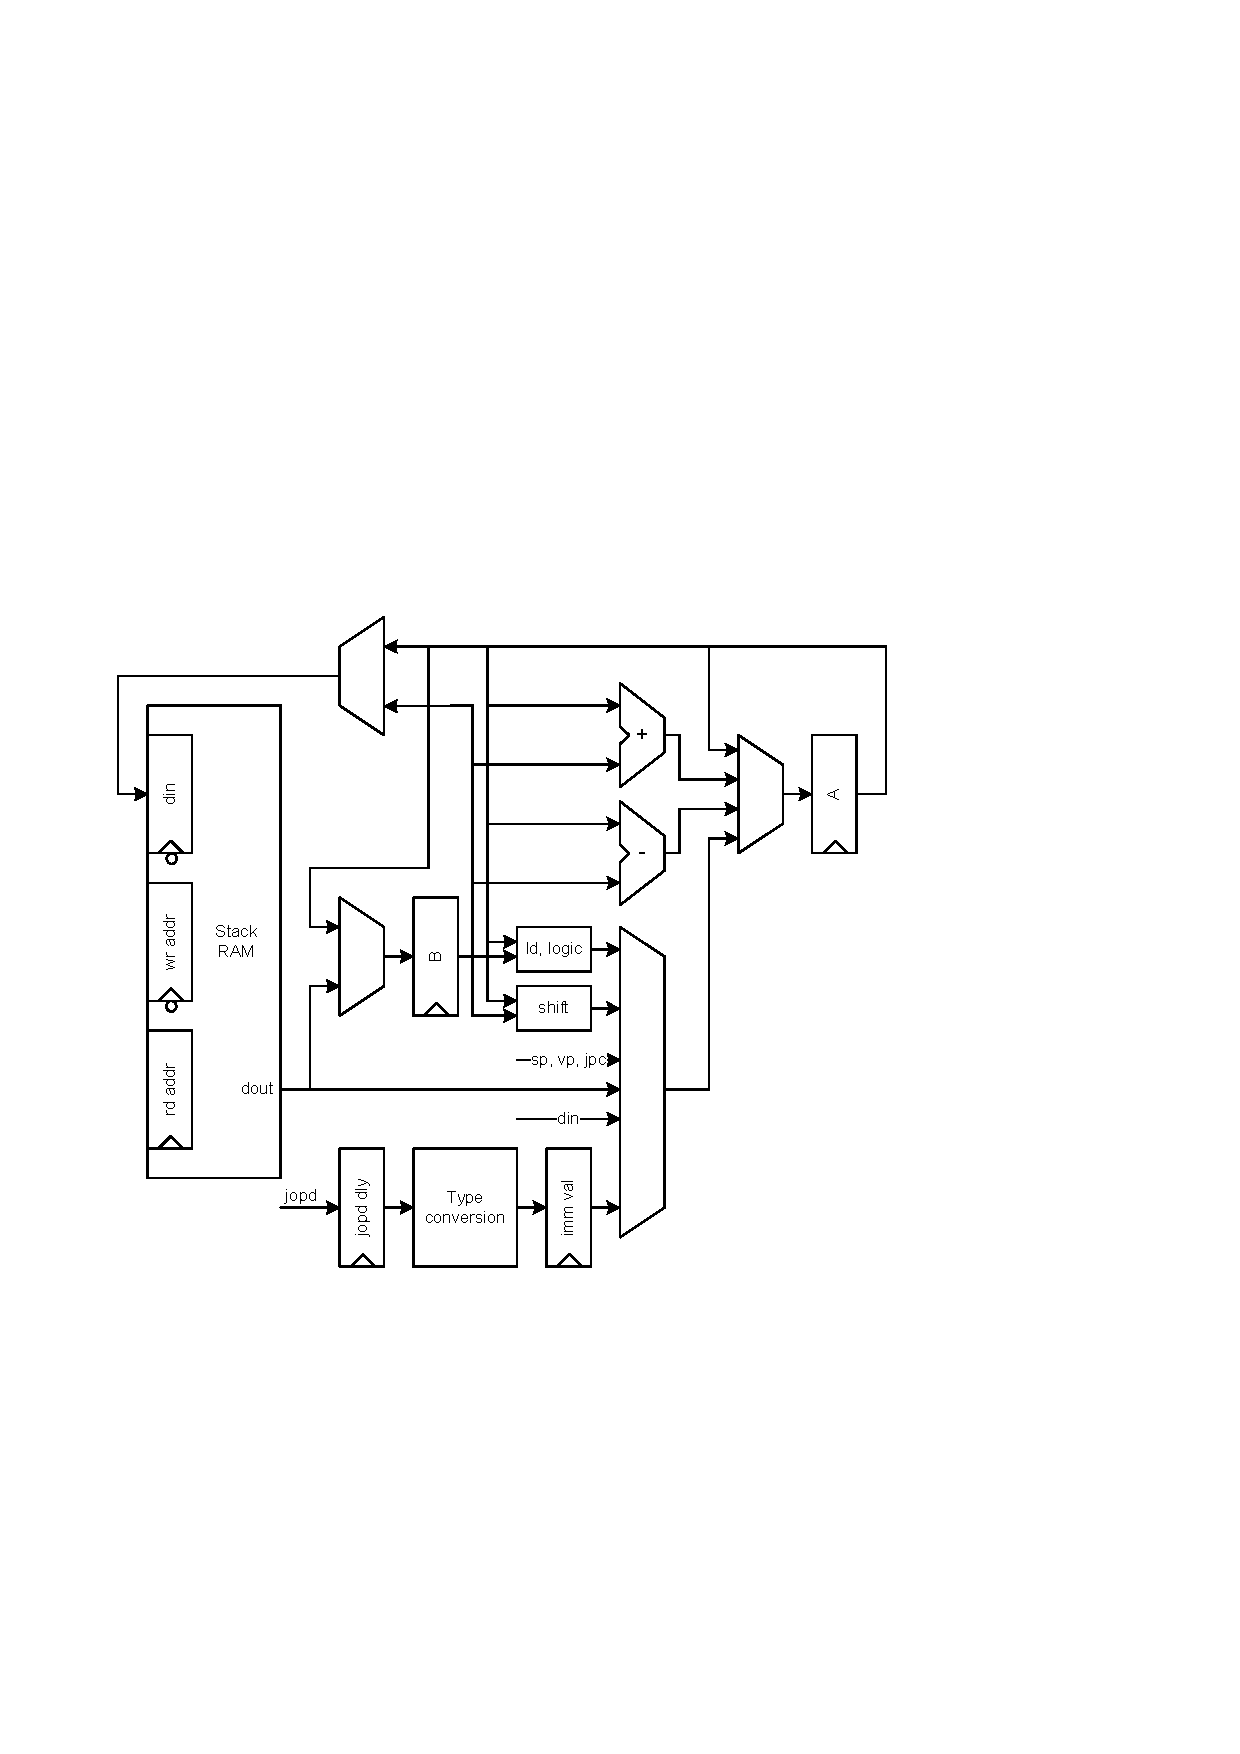
\includegraphics[scale=\picscale]{arch/arch_execute}
    \caption{Execution stage}
    \label{fig_arch_exe}
\end{figure}

Each arithmetic/logical operation is performed with registers
\emph{A} and \emph{B} as the source, and register \emph{A} as the
destination. All load operations (local variables, internal
register, external memory and periphery) result in a value being
loaded into register \emph{A}. There is therefore no need for a
write-back pipeline stage. Register \emph{A} is also the source for
the store operations. Register \emph{B} is never accessed directly.
It is read as an implicit operand or for stack spill on push
instructions. It is written during the stack spill with the content
of the stack RAM or the stack fill with the content of register
\emph{A}.

Beside the Java stack, the stack RAM also contains microcode
variables and constants. This resource-sharing arrangement not only
reduces the number of memory blocks needed for the processor, but
also the number of data paths to and from the register \nolinebreak
\emph{A}.

The inverted clock on data-in and on the write address register of
the stack RAM is used, for the same reason, as on the read address
register of the microcode ROM.

A stack machine with two explicit registers for the two topmost
stack elements and automatic fill/spill needs neither an extra
write-back stage nor any data forwarding. Details of this two-level
stack architecture are described in Section~\ref{sec:stack}.

%\subsection{Pipeline Example}
%
%\emph{\textbf{Show from Java code downto FPGA HW.}}
%
%Is in brown bock.

\subsection{Interrupt Logic}
\label{sec:interrupt}

Interrupts and (precise) exceptions are considered hard to implement
in a pipelined processor \cite{Hennessy02}, meaning implementation
tends to be complex (and therefore resource consuming). In JOP, the
bytecode-microcode translation is used cleverly to avoid having to
handle interrupts and exceptions (e.g., stack overflow) in the core
pipeline.

Interrupts are implemented as special bytecodes. These bytecodes are
inserted by the hardware in the Java instruction stream. When an
interrupt is pending and the next fetched byte from the bytecode
cache is an instruction (as indicated by the \emph{nxt} bit in the
microcode), the associated special bytecode is used instead of the
instruction from the bytecode cache. The result is that interrupts
are accepted at bytecode boundaries. The worst-case preemption delay
is the execution time of the \emph{slowest} bytecode that is
implemented in microcode. Bytecodes that are implemented in Java
(see Section \ref{subsec:flex:bc}) can be interrupted.

The implementation of interrupts at the bytecode-microcode mapping
stage keeps interrupts transparent in the core pipeline and avoids
complex logic. Interrupt handlers can be implemented in the same way
as standard bytecodes are implemented i.e.\ in microcode or Java.

This special bytecode can result in a call of a JVM internal method
in the context of the interrupted thread. This mechanism implicitly
stores almost the complete context of the current active thread on
the stack. This feature is used to implement the preemptive, fixed
priority real-time scheduler in Java \cite{jop:javasched}.

The main source for an interrupt is the $\mu$s accurate timer
interrupt used by the real-time scheduler. Hardware generated
exceptions, such as stack overflow or array bounds checks, generate
a system interrupt. The exception reason can be found in a register.

\subsection{Summary}

In this section, we have analyzed JOP's pipeline. The core of the
stack machine constitutes a three-stage pipeline. In the following
section, we will see that this organization is an optimal solution
for the stack access pattern of the JVM.

An additional pipeline stage in front of this core pipeline stage
performs bytecode fetch and the translation to microcode. This
organization has zero overheads for more complex bytecodes and
results in the short pipeline that is necessary for any processor
without branch prediction. This additional translation stage also
presents an elegant way of incorporating interrupts virtually
\emph{for free}.
